\section{Accelerating the detection of the preamble}
In the previous Hands-On, our demodulation chain required a component called the \textit{preamble detector} that actively seeks the preamble sequence located at the beginning of a packet by looking at the energy of each sample and accumulating it over time. When the accumulated value exceeded a threshold, the preamble was considered present and a given amount of samples were forwarded to the synchronization stage. This system allows to avoid unnecessary heavy computations as well as real-time operation. There are two drawbacks to this process. First, the threshold is not updated and increasing the gain of the RF front-end will increase the noise power, possibly going above the set threshold. Second, this preamble detection scheme requires a lot of computation, calculating and accumulating the energy of each sample. \\

As it operates continuously, it is best to move its functionality from software towards a specialized piece of hardware in order to improve its \textbf{energy efficiency and processing speed}. If we decide at one point to increase the packet rate of the overall transmission chain, this solution is more robust regarding packet misses. It is also further motivated by the fact that this block occurs at the very beginning of the processing chain, just after the low-pass filter. We will also change the behavior of the block by calculating the threshold based on the noise power and on a programmable margin coefficient. The accelerated block will therefore be called the packet presence detector (PPD). However, we only want to accelerate the energy detection step but still receive all samples in GNU Radio to be able to monitor the channel if needed. Therefore, the PPD will add a flag at the start of a packet when it has been detected. This flag corresponds to the value \texttt{0x7FF} which can not be practically reached by the LMS7002M chip.


\subsection{Design overview}
We implemented for you a packet presence detection module in SystemVerilog HDL\footnote{Although uncommon, it is possible to mix multiple HDL languages in a single design. For instance, the majority of the LimeSDR-Mini system is written in VHDL, but for your convenience we have written the PPD in SystemVerilog.}. First, open the Quartus project, \texttt{LimeSDR-Mini\_lms7\_lelec210x/LimeSDR-Mini\_lms7\_lelec210x.qpf}. If a message asking you for overwriting the database is printed, click "yes". With Quartus or any other code editor, you can then open the PPD design file located in\\ \texttt{LimeSDR-Mini\_lms7\_lelec210x/ip/packet\_presence\_detection/packet\_presence\_detection.sv}\\ and containing the following interfaces:
\begin{itemize}
    \item A clock and reset interface.
    \item A sink (input) streaming interface with data and valid signals.
    \item A source (output) streaming interface with data and valid signals.
    \item A custom static interface for configuration signals.
\end{itemize}
The PPD follows the low-pass filter in the receiver chain, as you have seen in previous hands-on. The filter, implemented using a FIR, is already included in the hardware design provided to you. Indeed, as a FIR is composed of multiply-and-accumulate operations, it can be easily accelerated in hardware. The  PPD module is integrated as a custom IP inside the same subsystem as the FIR, it therefore shares the same streaming interfaces\footnote{See pp 40-52 of \texttt{mnl\_avalon\_spec.pdf} on Moodle for details.}: the data bus is 24-bit wide with the MSBs and LSBs containing the samples of the I and Q channels respectively. In addition a valid signal is associated with the streaming data to indicate whether the data bus contains information of interest, or not. With the PPD, the goal is to produce an output valid signal that indicates if the complex magnitude of the data has reached a threshold.

\begin{figure}[h]
    \centering
    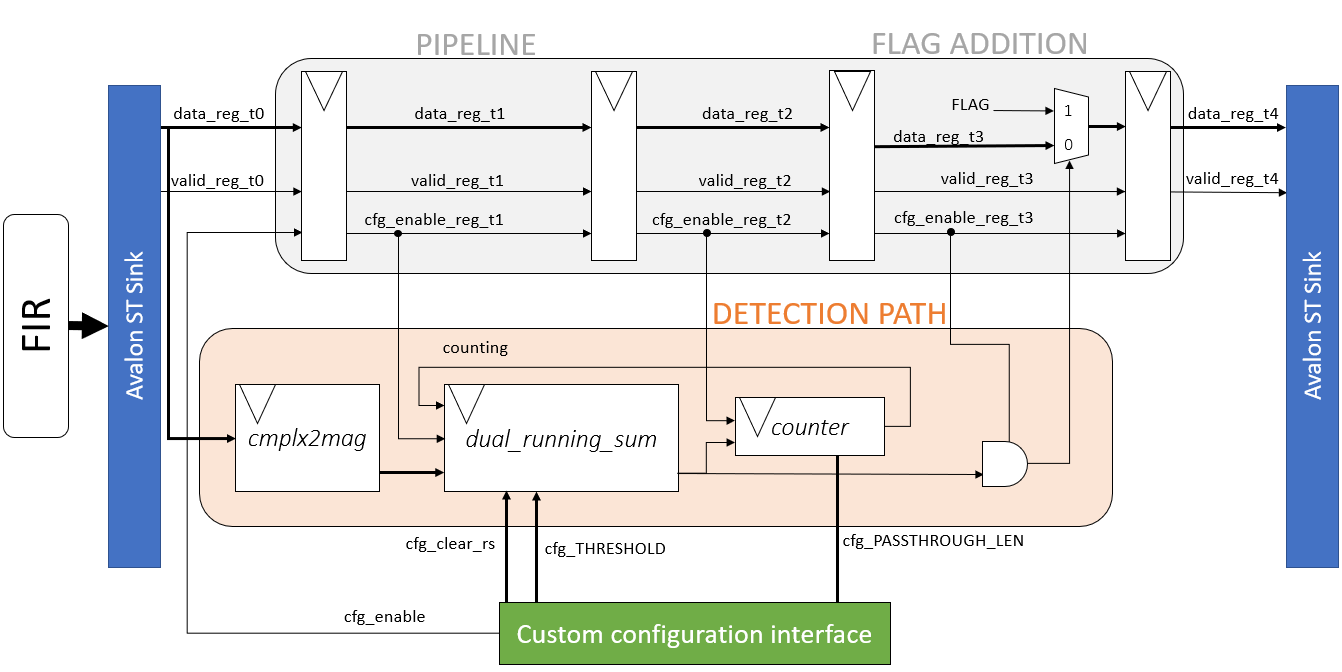
\includegraphics[width=\linewidth]{figures/packet_presence_detection.png}
    \caption{Hardware packet presence detector schematic}
    \label{fig:pd_schematic}
\end{figure}

\subsection{Packet presence detector schematic}
In Figure \ref{fig:pd_schematic} below you can find a schematic of the different modules that compose the PPD. As a reminder, the objective of this block is to add a flag at the start of a packet when a sufficient energy has been detected in the signal. It functions as follows:
\begin{enumerate}
    \item \textbf{Complex to magnitude: } The IQ samples are processed by a \textit{complex to magnitude} block which outputs the magnitude of the complex IQ vector.
    To do so, we calculate the magnitude as the square root of $I^2+Q^2$. As square-root function are difficult to implement in hardware logic, we are thus going to use a very simple and accurate algorithm. The estimate for the first quadrant of the trigonometric circle is drawn on Figure \ref{fig:cmplx2mag}. The mathematical formula is provided to you in Equation \ref{eq:1norm}\footnote{Further information can be found online: \url{https://en.wikipedia.org/wiki/Alpha_max_plus_beta_min_algorithm} and \url{http://dspguru.com/dsp/tricks/magnitude-estimator/}.}.

    \begin{equation}
        |z| = \frac{min(|I|,|Q|)}{4} + max(|I|,|Q|)
        \label{eq:1norm}
    \end{equation}

    \begin{figure}[h]
        \centering
        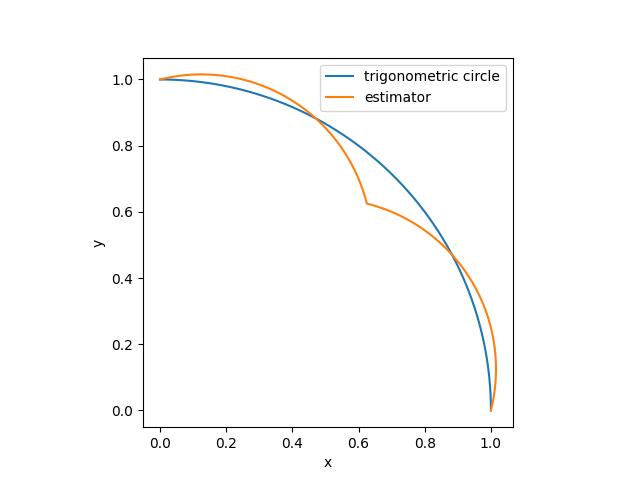
\includegraphics[width=0.45\linewidth]{figures/trigo.png}
        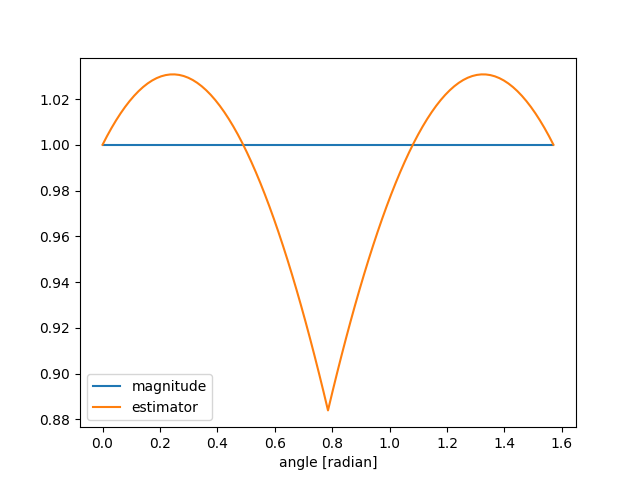
\includegraphics[width=0.45\linewidth]{figures/angle.png}
        \caption{Complex Magnitude Estimator output in x-y coordinates (left) or polar coordinates (right) for input points of the trigonometric circle.}
        \label{fig:cmplx2mag}
    \end{figure}

    \item \textbf{Dual running sum: } The estimated complex magnitude of the samples is then averaged over multiple samples by two moving average filter of different length in series, a short-term sum and long-term one. They are implemented by forwarding input samples in  memory-based \textit{delay lines}, developped by Altera.

    \begin{align}
            y[n] = \sum_{k=0}^{N-1}\left|x[n-k]\right|
    \end{align}

    At each clock cycle an accumulator adds and substracts the first and last magnitude values stored in the delay line to its content. This structure is more efficient than the general FIR because we know each tap is equal to one, we therefore only need two adders.

    \begin{align}
            y[n+1] = y[n] + \left|x[n]\right| - \left|x[n-N+1]\right|
    \end{align}

    The two moving average filters have two different functions. The first one, the short-term sum, receives the sample magnitudes first and its delayed output value are then forwarded to the long-term sum. This longer delay line is used to evaluate the noise power.

    \begin{figure}[h]
        \centering
        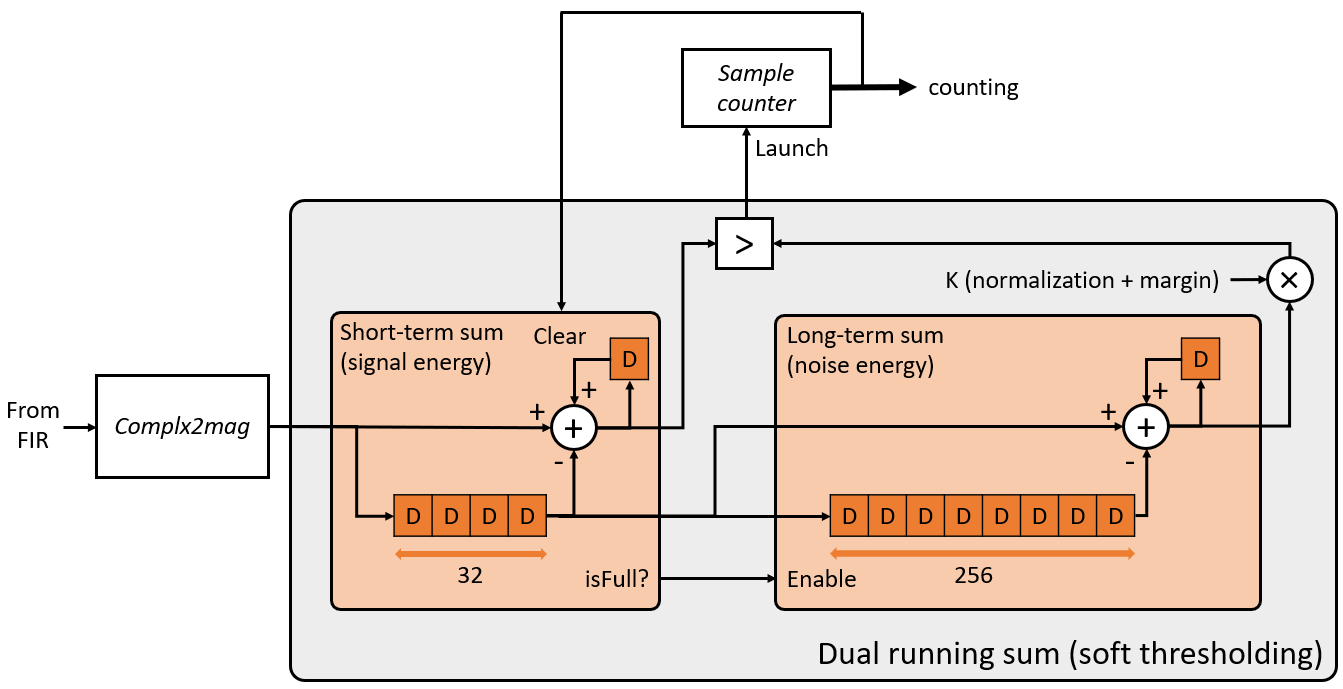
\includegraphics[width=\linewidth]{figures/dual_running_sum_block.png}
        \caption{Architecture of the dual running sum}
        \label{fig:dual_runnign_sum}
    \end{figure}

    The overall architecture of the dual running sum is shown in Fig. \ref{fig:dual_runnign_sum}. If no packet is being received, the samples contain only noise. They pass through the short-term sum and then the long-term one. Both their accumulator can then be seen as noise power estimations.  When a packet arrives, possibly with  higher energy than the noise, the corresponding samples first enter the short-term sum. Its accumulator value therefore increases and might at one point exceed the accumulator value of the long-term sum, which contains only noise samples. At this point, a packet is considered present and a launch signal is triggered.

    To be noted, when a packet is detected and the counter (next block) is enabled, we clear the short-term sum and disable the long-term one, to avoid any retriggering or corruption of our noise evaluation by packet samples.


    \item \textbf{Counter :} This block receives the launch signal of the previous block. This counter block is used to count the samples when the threshold has been reached and avoid triggering a start flag multiple times inside a single packet. During the sequence, a \texttt{running} signal indicates the state of the counter. This signal is used to clear the short-term sum of the dual running sum. The number of samples that are passed is configurable.

    \item \textbf{Flag addition :} A multiplexer is used at the end to replac a sample with a flag, here $I=$\texttt{0x7FF} and $Q=$\texttt{0x7FF}, when the launch signal is triggered.

\end{enumerate}


In order to reduce the length of the critical path between registers, we use a paradigm called \textit{pipelining}. In short, we divide the operations of the PPD into several stages with similar length. As the critical path in this configuration is much shorter, it allows to operate the circuit at a higher frequency. In return, the additional registers add area and energy consumption to the design. It also requires to forward control signals in the pipeline and it can add complexity (see \textit{Control Path} in Figure \ref{fig:pd_schematic}). You will learn the concept of pipelining in details when studying the \textit{pipelined processor} in the course of \texttt{LELEC2531}.

Try to understand the SystemVerilog implementation of those blocks with respect to their theoretical behavior. Pay particular attention to the bus width of intermediate signals, they are computed in order to systematically avoid any overflow of intermediate values!


\subsection{Modification and simulation of the PPD}


We will first ask you to make some modifications to the dual running sum, more specifically to the comparison between the short- and long-term sum results. In order to make it adaptative from GNU Radio, we will use the \texttt{cfg\_THRESHOLD} signal of the packet presence detection module to multiply the result of the long-term sum before comparing it to the short-term sum result. This allows to be more selective regarding the signal-to-noise ratio required to detect the packet. Increasing its value will limit the risk of false alarm due to noise but make your system less sensitive. In short, with this parameter set to 10, the PPD would require a signal magnitude 10 times higher than the noise one to trigger a detection. However, we should also normalize the short-term and long-term result with respect to the delay line length, the second one being here eight times longer than the first. Overall, we ask you to implement the multiplication shown in Figure \ref{fig:dual_runnign_sum}. In the SystemVerilog code, go to the line 199. We ask you to implement both the normalization, i.e. division by eight, and the multiplication operation on the same line. Note that the \texttt{cfg\_THRESHOLD} signal is connected to the \texttt{K} input of the dual running sum module.


\begin{bclogo}[couleur = gray!20, arrondi = 0.2, logo=\bcquestion]{Division by eight}
    \begin{itemize}
        \item Performing multiplications and divisions is much more complex than simple additions. However, when performing operations with values that are power-of-two, things always seem easier. What would be an efficient way to perform the division by eight?
        \item The order in which the two operations are performed, here the multiplication by K and division by eight, would normally have no importance. Is it the case here? Which operation should be performed first and why?
    \end{itemize}
\end{bclogo}

Once you have implemented this function, we should now test the PPD. We have developped a testbench for you, and we will use ModelSim to verify the PPD behavior before deploying it into the complete system. A few python scripts located at \texttt{ip/packet\_presence\_detection/testbench/python} allow you to generate input vectors for the PPD and compare the testbench output with an expected result obtained with python:

\begin{enumerate}
    \item \texttt{1\_input\_gen.py} : generates input vectors and export them as input vector of the PPD HDL implementation.

    \item To generate the testbench, we will use the \textit{Platform Designer}. It allows the interconnection of multiple blocks of a digital design with a more intuitive user interface. Open the \textit{Platform Design} using the shortcut highlighted in Figure \ref{fig:quartus_platform_designer}. Open the \texttt{packet\_presence\_detection\_tb\_gen.qsys}, and go in \textit{Generate} in the upper left corner, then \textit{Generate Testbench System}. Change the path to \texttt{LimeSDR-Mini\_lms7\_lelec210x/ip/packet\_presence\_detection/} and click on \textit{Generate}. To execute the testbench, open ModelSim and change the working directory to\\ \texttt{ip/packet\_presence\_detection/testbench}. Then run \texttt{do run\_sim.tcl} in order to compile and launch the simulation.

\begin{figure}[H]
    \centering
    
\includegraphics[scale=0.7]{figures/quartus_toolbar.PNG}
    \caption{Toolbar of Quartus. The Platform Designer shortcut is highlighted in yellow.}
    \label{fig:quartus_platform_designer}
\end{figure}

    \item \texttt{2\_compare} : when the SystemVerilog testbench has been executed, compares the input data samples to the output of the PPD, plotting them. Is the PPD working as expected? Do not hesitate to ask your questions to a teaching assistant to ensure you fully understand where and why flags are added.
\end{enumerate}

Once you have analysed the results, we will propagate the changes you made to the complete system that will be flashed on the FPGA. Remember we only modified the IP, we now need to propagate those changes to the actual design. In the \textit{Platform Designer}, open the \texttt{lms\_dsp.qsys} design. Nothing has to be done except clicking \textit{"Generate HDL ..."} on the bottom right of the window and update the path to
\texttt{LimeSDR-Mini\_lms7\_lelec210x/lms\_dsp/} if it is not made automatically. Then press on \textit{"Generate"}. The changes you made locally to the PPD have now been propagated. In the Platform Designer, you can quickly observe the structure of the \textit{lms\_dsp} block, with the FIR, the packet presence detection and the different Avalon Streaming Interface.

You can now compile your design and observe the resource and timing report. Be careful when launching a compilation in Quartus, a window may ask you to update the project revision. Answer \textit{"NO"}.

\begin{bclogo}[couleur = gray!20, arrondi = 0.2, logo=\bcattention]{MAX 10 Device Support might not be installed}
    The support for the FPGA device we use might not be installed in the Quartus you have, which will lead to errors in the compilation. The installation instructions are provided in the wiki of the course.

\end{bclogo}

\subsection{Timing and ressource analysis}

As you have seen in course, an important aspect of digital design is to ensure that your design meet both the resource and timing requirements. Indeed, long combinatorial logic path can lead to setup or hold constraints violations. Now that the design has been compiled, you can check the compilation report using the shortcut highlighted in Figure \ref{fig:compilation_report_button}.

\begin{figure}[h]
    \centering
    
\includegraphics[width=\linewidth]{figures/Compilation_report_button.PNG}
    \caption{Toolbar of Quartus. The Compilation Report shortcut is highlighted in red.}
    \label{fig:compilation_report_button}
\end{figure}


In the \textit{"Flow Summary"} tab, the resource utilisation is reported. Observe for instance the number of embedded multipliers that are employed. Moreover, in the \textit{"Analysis \& Synthesis/Timing Analyzer"} tab, you can see the results for the different corners, constraints violations being highlighted in red. Try to identify the faulty clock involved. In the different summary proposed, you can right click on a clock and select \textit{"Report Timing... (In Timing Analyzer UI)"}. In the opened window, just press \textit{"Report Timing"} at the bottom. Those steps are depicted in Figure \ref{fig:report_timing_analyzer}. You can now analyze the most critical path implying the selected clock, as well as the logic cells involved. Try to link the critical path to the RTL design. It should involve a signal starting in the dual running sum module. An easy fix is here to add a register in the path to break in two. This will delay the launch signal by one clock cycle, which is not problematic. \textbf{If you make a modification to the verilog of the PPD, you need to regenerate it in the Platform Designer}.

\begin{figure}[h]
    \centering
    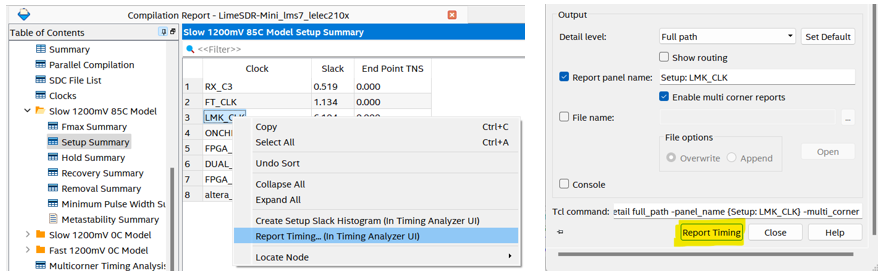
\includegraphics[width=\linewidth]{figures/Report_Timing_Analyzer.png}
    \caption{Steps to analyze the most critical path on a given clock.}
    \label{fig:report_timing_analyzer}
\end{figure}

Moreover, we prevented \textbf{register retiming} which allows the synthesis tool to balance the combinatorial logic across registers when it does not affect the system behaviour. This helps on meeting the timing requirements by offloading parts of long combinatorial path. To enable this setting, go in \textit{"Assignments/Settings/Compiler Settings"} on Quartus and uncheck the \textit{"Prevent register retiming"} box.

Before relaunching a compilation, ask for an assistant to check your modifications, to avoid wasting precious synthesis time. Done? Now relaunch a compilation and analyze the results. Again, if a window asks you to update the project revision, answer \textit{"NO"}. Is there still a timing constraint violation? Can you still link the most critical path to the HDL design?

To analyse the ressource used by the design, you can look at the \textit{Hierarchy} tab in the \textit{Project Navigator}. More than navigating through the design, you can also look at the ressource used by each module. Analyse the resource usage of the PPD, more specifically the memory bits and the DSP.
\begin{comment}
\subsection{From Euclidean norm to Absolute-value norm}

In order to meet the timing requirements, another solution is to use a less complex estimation of the IQ samples magnitude. We are thus going to use a very simple and accurate algorithm that does not have the burden of implementing the complex logic of \textit{integer multiplication}. The estimate for the first quadrant of the trigonometric circle is drawn on Figure \ref{fig:cmplx2mag}. We ask you to implement it in System Verilog, the mathematical formula being provided to you in Equation \ref{eq:1norm}\footnote{Further information can be found online: \url{https://en.wikipedia.org/wiki/Alpha_max_plus_beta_min_algorithm} and \url{http://dspguru.com/dsp/tricks/magnitude-estimator/}.}. Your modification of the \texttt{cmplx2mag} module must be done in the \texttt{USER CODE} parts, which goes from line 45 to 52 and on line 210. As we were performing two multiplications and one addition in the previous algorithm ($I^2+Q^2$), the data bus at the output of the \textit{cmplx2mag} module was specified as twice the input data bit width (due to multiplication) plus one (due to the addition). This is specified on line 210, do not forget to adapt it for the new algorithm. In the next step, you are going to make a behavioral simulation of you implementation to validate it.

\begin{equation}
    |z| = \frac{min(|I|,|Q|)}{4} + max(|I|,|Q|)
    \label{eq:1norm}
\end{equation}

\begin{figure}[h]
    \centering
    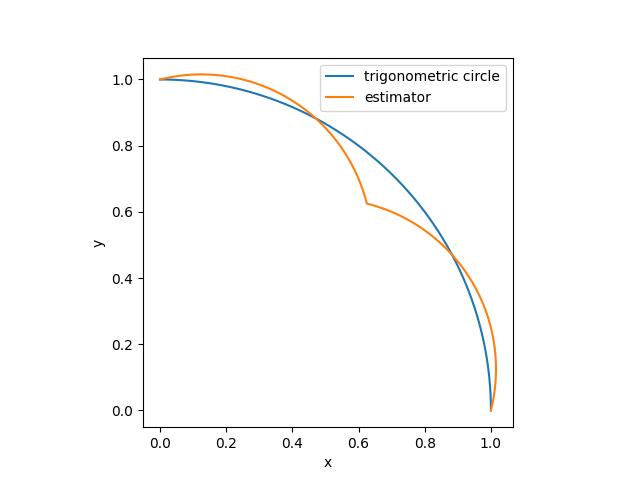
\includegraphics[width=0.45\linewidth]{figures/trigo.png}
    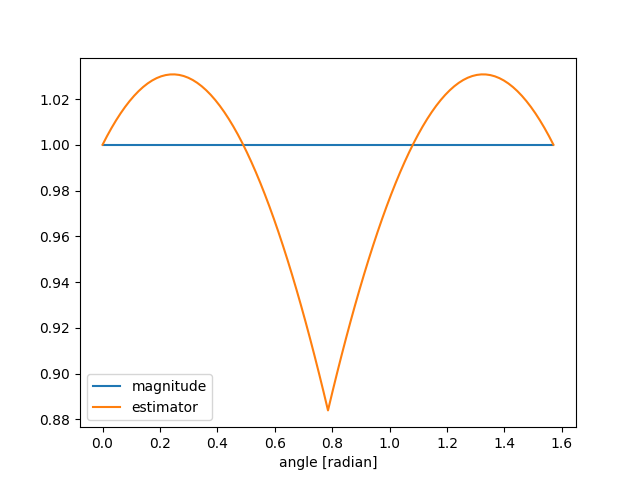
\includegraphics[width=0.45\linewidth]{figures/angle.png}
    \caption{Complex Magnitude Estimator output in x-y coordinates (left) or polar coordinates (right) for input points of the trigonometric circle.}
    \label{fig:cmplx2mag}
\end{figure}


Now that you have a functional design for the PPD with the Absolute-value norm, we can perform a synthesis of the complete design. Do not forget to propagate your change by regenerating the HDL via the Platform Designer. Observe the resource usage and the timing report, is there still a timing constraint violation?

\end{comment}
